\chapter{\textit{go-safer}: Detecting Unsafe Misuses}\label{ch:go-safer}

Another major contribution of this thesis is the development of a Go Vet-style, open-source linter tool.
It can identify some of the unsafe code patterns.

\begin{figure}[ht]
    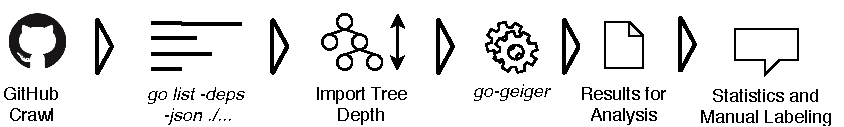
\includegraphics[width=\textwidth]{assets/figures/study-methodology.pdf}
    \caption{Overview of our Study Methodology}
    \label{fig:study-methodology}
\end{figure}



\section{Design}

Top-level approach
Usage example
Publication

\begin{figure}[!t]
    \vspace{2mm}
    \centering
    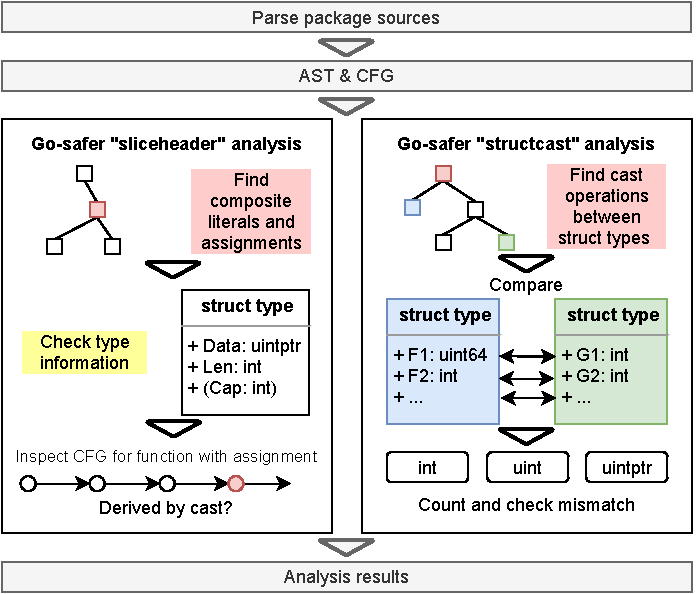
\includegraphics[width=0.48\textwidth]{gfx/figures/go-safer-architecture.pdf}
    %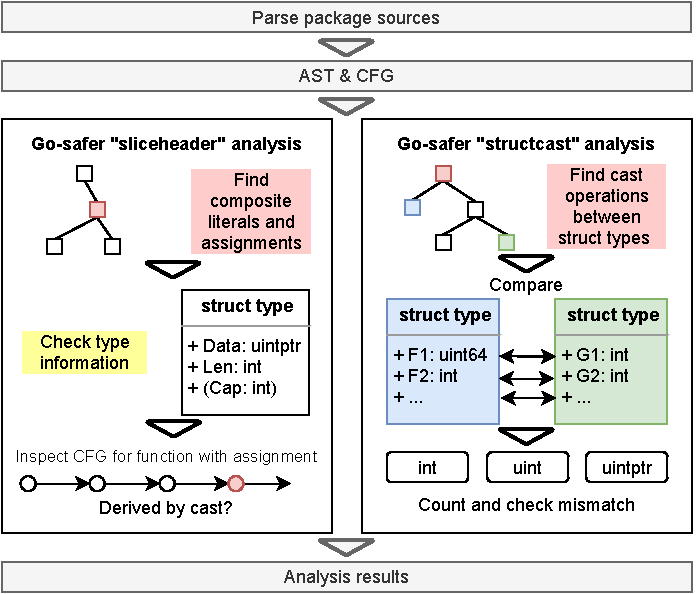
\includegraphics[width=0.45\textwidth]{gfx/figures/go-safer-architecture.pdf}
    \caption{Architecture of \toolSA{} static code analysis tool}
    \label{fig:safer-architecture}
    %\vspace{-14pt}
\end{figure}



\section{Implementation}

Go vet analysis pass infrastructure
Low-level details
Verification with tests


\section{Evaluation}

\subsection{Labeled Usages}

Precision, Recall, calculated using manually labeled usages data set


\subsection{Case Studies}

Manual inspection of some projects, used to calculate precision / recall of go-safer


\subsection{Comparison with Existing Tools}

Go vet / golint
